\label{user-login}
\subsubsection{Purpose}
Any subscribed user can login to use myTaxiService services.
The system requires the user to provide nickname and password, or e-mail and password, to log in correctly.

If the user doesn't remember his password, a new one is sent to the user's e-mail address. If the user clicks on the link in the e-mail, the password is reset and, as soon as he logs in, the system asks him to choose a new one. 



\subsubsection{Scenario 1}
Bob opens the home page of myTaxiService on the web and clicks on ``login''. 
he's asked to enter the nickname or the e-mail and the password. He doesn't recall his nickname, so he enters the registration e-mail and the password. He clicks on ``enter''. 
Everything is correct so he can access to the services as a logged user.

\subsubsection{Scenario 2}
Alice opens the home of myTaxiService page on web and clicks on ``login''.  
She is asked to enter the nickname or e-mail and the password.
She enters nickname and password and selects ``enter''. However, the entered password isn't correct so the system asks her to re-enter it. 
After some failed attempts she select ``password forgot''.
The system sends to her a new password via e-mail. She enters that one and the access is permitted, but before successfully ending the login the system requires her to change the password immediately. 
Alice changes her password and finally logs in to the services.

\begin{figure}
\begin{center}
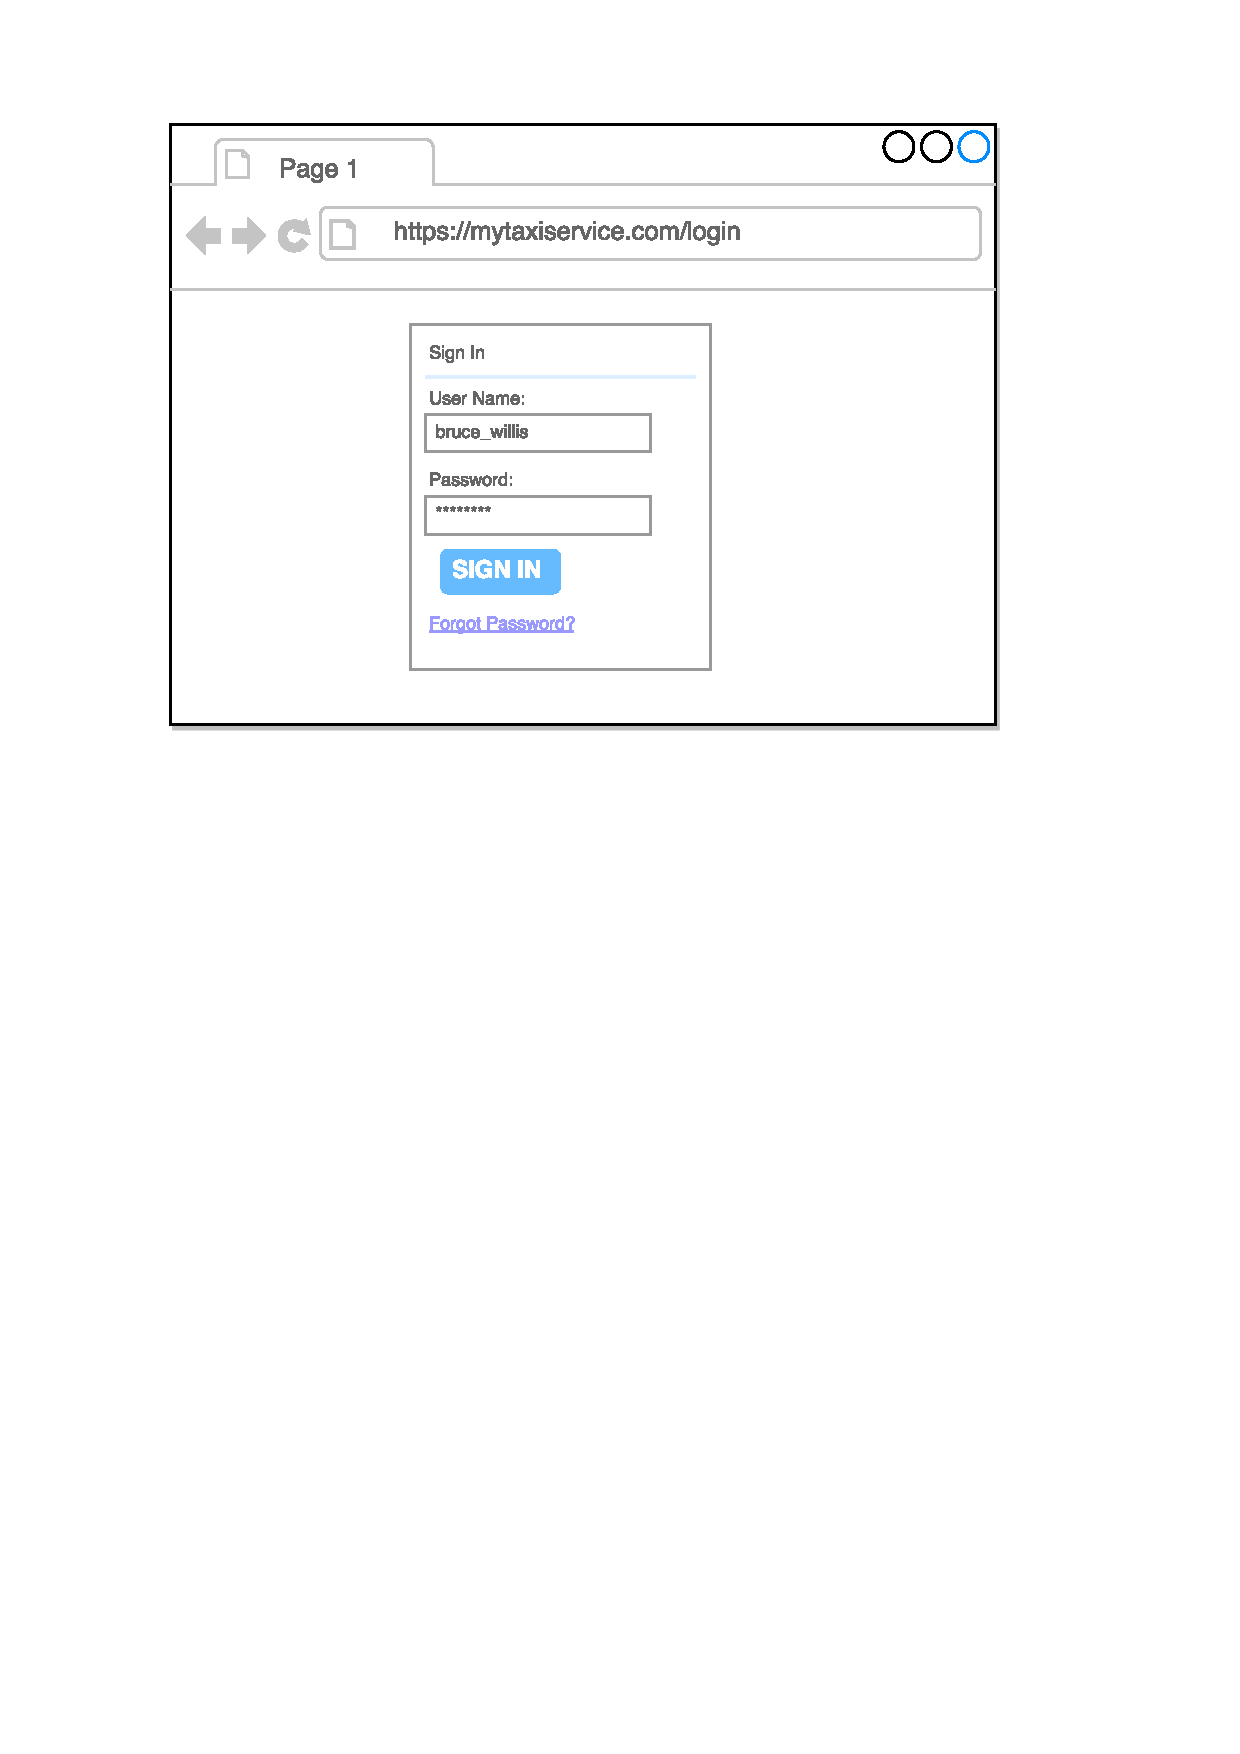
\includegraphics[width=0.7\textwidth]{mockup/Login_browser.pdf}
\caption{Concept of the login webpage.}
\label{fig:mockup-login}
\end{center}
\end{figure}

\subsubsection{Use case}
The use case for user login is shown in~\autoref{usecase-login}.

\begin{table}
\begin{center}
\begin{tabular}{| l | p{0.6\textwidth} |}
\hline
Actor & Registered passenger or taxi driver \\
\hline
Goal & Goal ~\ref{g-login}
\\
\hline
Input condition & The user, already registered, chooses to login.  \\
\hline
Event Flow & \begin{enumerate}
	\item The user selects ``login''.
	\item The login page is shown. \label{load-login}
	\item The user enters his/her credentials.
	\end{enumerate}
\\
\hline
Output condition & The system tells the user that he/she has been successfully logged in.
It is loaded the main page where the user can choose one of the myTaxiService options. \\
\hline

Exception & If the username/e-mail or password entered are wrong, the system notifies the user and the login page is reloaded (step~\ref{load-login} of Event Flow): the login has failed. 

	
 \\
\hline
\end{tabular}
\end{center}
\caption{Use case for user login.}
\label{usecase-login}
\end{table}





\subsubsection{Response sequence}
The response sequence is illustrated in figure \ref{fig:sequence-login}.
\begin{figure}
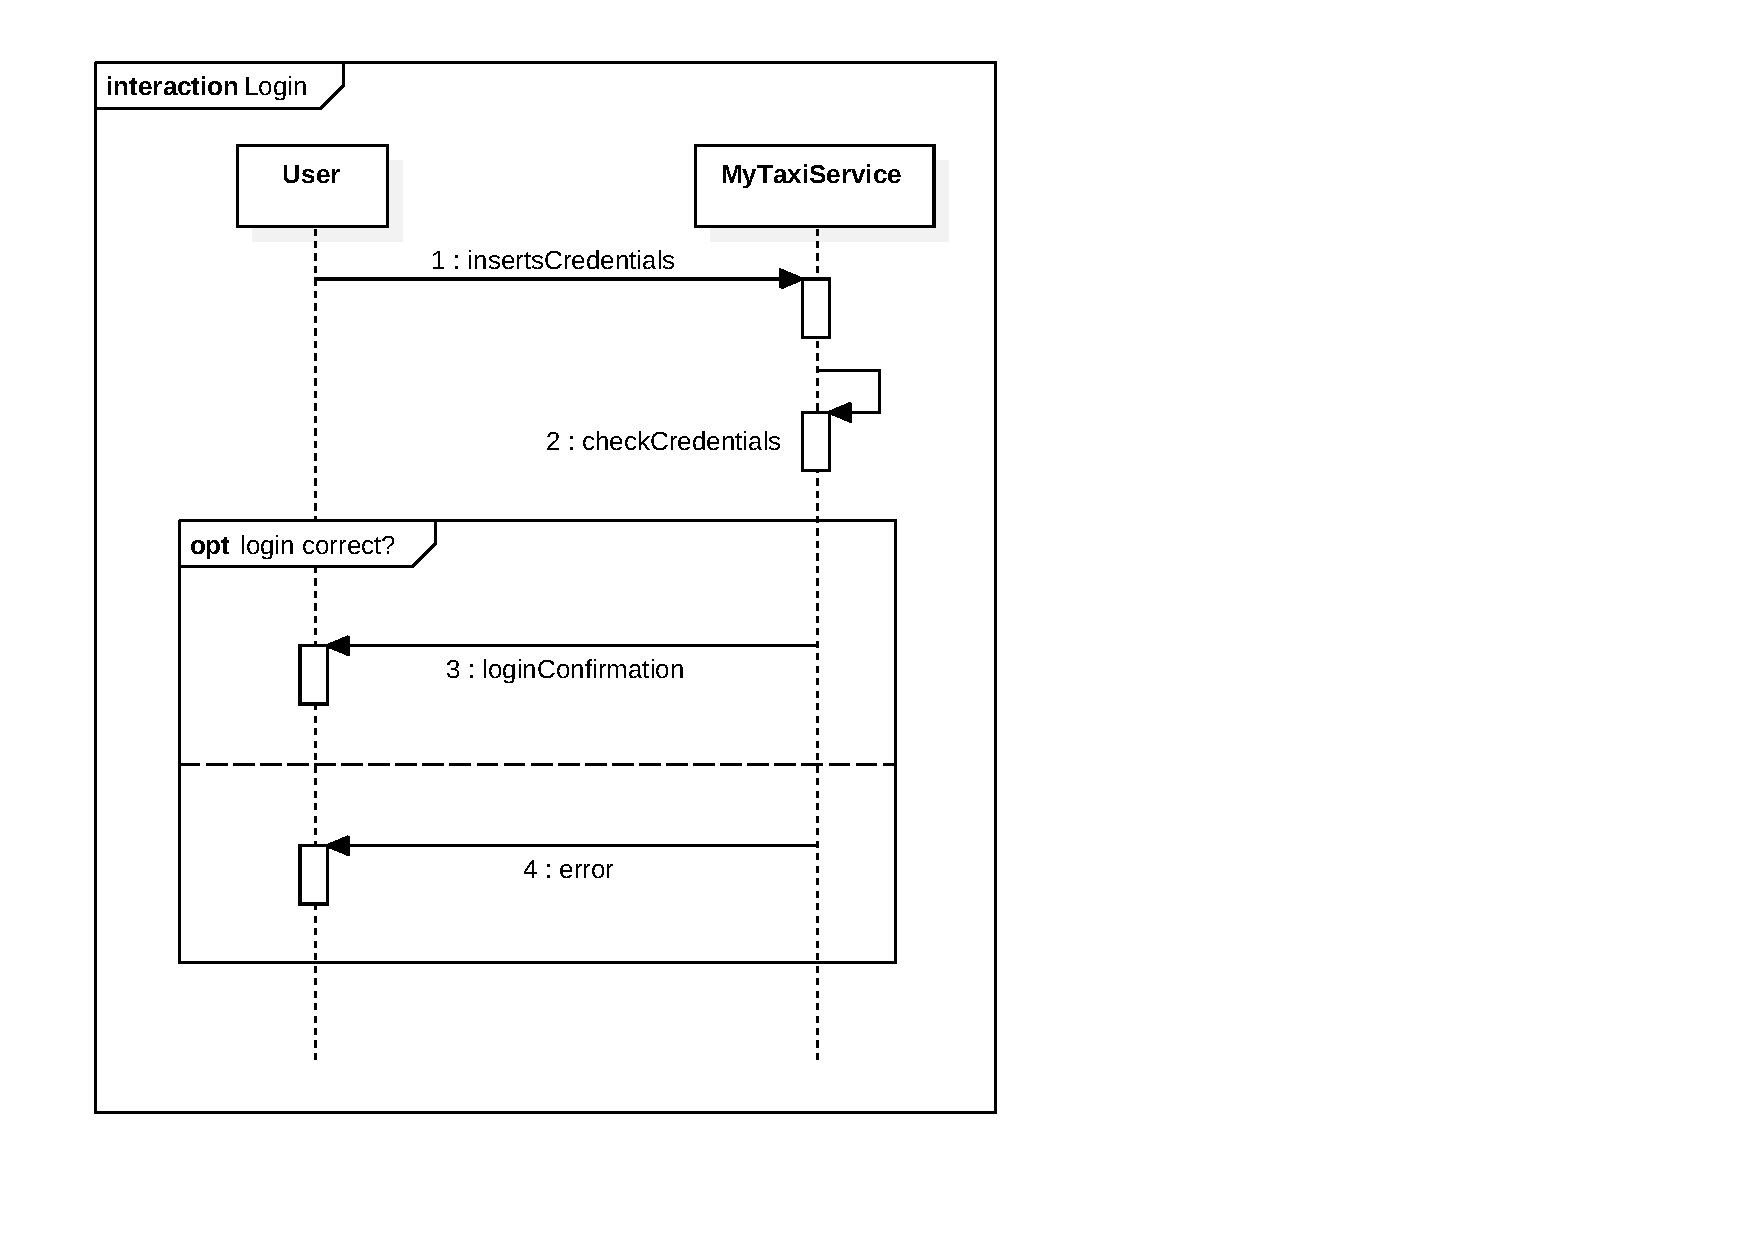
\includegraphics[width=\textwidth]{diagrams/sequence_login.pdf}
\caption{Sequence diagram of a user login.}
\label{fig:sequence-login}
\end{figure}

\subsubsection{Associated functional requirements}
\begin{enumerate}
    \item In order to log in, the user must insert either a nickname, or the registration e-mail, but not both.
    \item On login, the system must grant to the user access to his/her account if and only if the following conditions are met:
    \begin{enumerate} 
    	\item The inserted nickname corresponds to a username of an existing user, or the inserted e-mail corresponds to the registration e-mail of an existing user.
	\item The inserted password is the same of that of the user identified above.
    \end{enumerate}
    \item The system sends an e-mail after the ``password forgot'' button is selected.
    \item The system reset the user's password only after the link on e-mail is clicked.
    \item If the password entered is wrong a new attempt can be made only 10 seconds later.
  
\end{enumerate}